\section{Metodologia}%
\label{sec:metodologia}

A fim de conduzir este trabalho, foi realizada uma pesquisa bibliográfica sobre \glspl{ga} e suas variações, o que possibilitou a compreensão do funcionamento desses algoritmos e a identificação de aspectos relevantes para a análise de sua performance.
Assim, foram escolhidas duas funções de benchmark dentre as disponíveis no pacote \gls{opfunu}~\cite{opfunu_software}, uma convexa e outra não convexa.

\subsection{Operadores}

O objetivo central desta pesquisa é avaliar diferentes operadores de seleção e \gls{crossover}, com a intenção de entender como essas variações impactam os resultados dos experimentos.
Para isso, foram escolhidos os seguintes operadores de seleção: roleta e torneio --- o qual foi testado com diferentes valores de \(K\), que representa a proporção de indivíduos selecionados para o torneio dentre a totalidade da população.
Além disso, foram escolhidos os operadores de \gls{crossover} de um ponto e aritmético.

Embora inicialmente o escopo do trabalho não contemplasse a introdução de mutações, foi necessário incluir alguma chance de mutação para evitar problemas de convergência prematura das soluções, o que poderia limitar significativamente a qualidade dos resultados obtidos.

Assim, foram realizados testes preliminares com diferentes métodos de mutação disponíveis no pacote \gls{mealpy}~\cite{mealpy_software}.
Os resultados desses revelaram que algumas técnicas, como \texttt{scramble} e \texttt{inverted}, eram incompatíveis com certas combinações de operadores --- como a combinação de seleção por roleta com crossover de um ponto.

Em contraste, a mutação do tipo \texttt{flip} mostrou-se bastante razoável em termos de tempo de execução e resultados obtidos, independentemente da combinação de operadores utilizada (roleta, torneio, crossover de um ponto e crossover aritmético).
Dessa forma, foi selecionada a mutação \texttt{flip} em todas as execuções do experimento.

\subsection{Funções objetivo}

Ademais, foi necessário ultrapassar os limites do escopo originalmente estabelecido também no que se refere ao número de dimensões avaliadas.
O objetivo inicial era analisar as funções em 2 e 10 dimensões, o que não constitui uma limitação da biblioteca \gls{mealpy}.
Entretanto, os arquivos que baseiam o pacote \gls{opfunu} apresentam as funções objetivo disponíveis em apenas cinco configurações: 10, 20, 30, 50 e 100 dimensões.

Levando em conta que se esperava que as execuções para duas dimensões permitissem a visualização gráfica do espaço de busca delimitado pelas funções, e que tal artefato não pôde ser gerado pelo software, foram inclusos os gráficos gerados por \citeonline{cec2014}.
Dessa forma, optou-se por avaliar as funções em 10 e 20 dimensões, que são os valores mais próximos daqueles inicialmente planejados.

As duas funções objetivo escolhidas para a realização dos experimentos foram \gls{f1}, que é convexa e cuja representação gráfica é apresentada na \autoref{fig:f1}, e \gls{f5}, que é não convexa e cuja representação gráfica é apresentada na \autoref{fig:f5}.

\begin{figure}[!ht]%
    \centering
    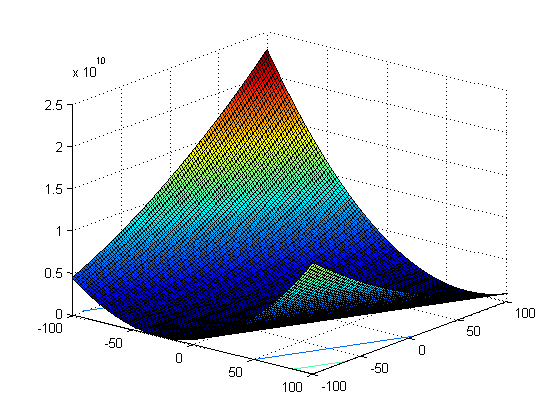
\includegraphics[scale=0.5]{img/f1.png}
    \caption{Mapa 3D para a função \glsentryfull{f1} em duas dimensões. Fonte: \citeonline{cec2014}.}%
    \label{fig:f1}
\end{figure}

\begin{figure}[!ht]%
    \centering
    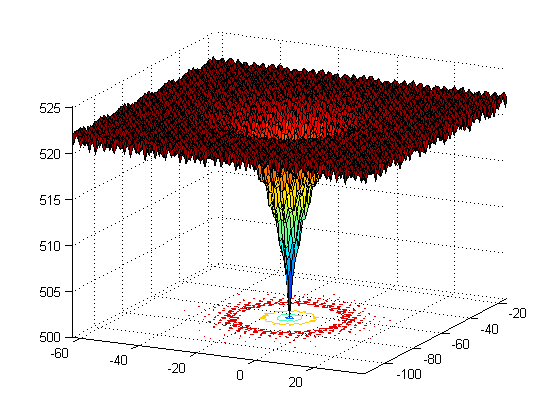
\includegraphics[scale=0.5]{img/f5.png}
    \caption{Mapa 3D para a função \glsentryfull{f5} em duas dimensões. Fonte: \citeonline{cec2014}.}%
    \label{fig:f5}
\end{figure}

\subsection{Configuração dos experimentos}

São apresentadas as constantes bem como os parâmetros escolhidos para a realização dos experimentos.

\subsubsection{Constantes}

Dado o escopo do trabalho, foram estabelecidas algumas constantes utilizadas em todos os experimentos realizados, as quais estão listadas na \autoref{tab:constantes}.

\begin{table}[htb]
    \center%
    \begin{tabular}{l l}
        \bottomrule
        \textbf{Constant}    & \textbf{Value} \\ \midrule
        Target               & Min            \\ \midrule
        Population size      & 50             \\ \midrule
        Crossover rate       & 90\%           \\ \midrule
        Mutation             & Flip           \\ \midrule
        Mutation rate        & 5\%            \\ \midrule
        Elitism rate (best)  & 10\%           \\ \midrule
        Elitism rate (worst) & 30\%           \\ \midrule
        Epochs               & 10000          \\ \toprule
    \end{tabular}
    \caption{Constantes utilizadas nos experimentos.}%
    \label{tab:constantes}
\end{table}

Todas as funções tem objetivo de minimização.
Cada gene dos indivíduos da população é representado por um número real entre -100 e 100.
A população inicial é gerada de forma aleatória dentro deste intervalo.
Seu tamanho se mantém fixo ao longo de todas as gerações, em 50 indivíduos.

O operador de \gls{crossover} é aplicado com uma taxa de 90\%, de forma que o método escolhido é parte das variáveis analisadas.
A mutação é aplicada com uma taxa de 5\%, e o método de mutação escolhido é o \texttt{flip}.

O elitismo é aplicado em 10\% dos melhores indivíduos e em 30\% dos piores.
A execução de cada iteração é realizada por 10000 gerações, ou épocas.

\subsection{Variáveis}

As variáveis analisadas nos experimentos se tratam dos operadores de seleção, que podem ser roleta ou torneio --- em que se varia a proporção da população selecionada para participar do torneio (10\%, 20\%, 30\%, 40\%, 50\%) ---, e do operador de \gls{crossover}, que pode ser de um ponto ou aritmético.

A compilação das variáveis resulta em 12 combinações possíveis, que são listadas na \autoref{tab:variaveis}, além das execuções com 10 e 20 dimensões, o que totaliza 24 experimentos para cada função objetivo.

\begin{table}[!ht]
    \center%
    \begin{tabular}{|l|l|l|}
        \bottomrule
        \multirow{2}{*}{Dimensions number} & \multicolumn{2}{l|}{10}                                 \\ \cline{2-3}
                                           & \multicolumn{2}{l|}{20}                                 \\ \hline
        \multirow{6}{*}{Selection}         & \multicolumn{2}{l|}{Roulette}                           \\ \cline{2-3}
                                           & \multicolumn{1}{l|}{\multirow{5}{*}{Tournament}} & 10\% \\ \cline{3-3}
                                           & \multicolumn{1}{l|}{}                            & 20\% \\ \cline{3-3}
                                           & \multicolumn{1}{l|}{}                            & 30\% \\ \cline{3-3}
                                           & \multicolumn{1}{l|}{}                            & 40\% \\ \cline{3-3}
                                           & \multicolumn{1}{l|}{}                            & 50\% \\ \hline
        \multirow{2}{*}{Crossover}         & \multicolumn{2}{l|}{One point}                          \\ \cline{2-3}
                                           & \multicolumn{2}{l|}{Arithmetic}                         \\ \toprule
    \end{tabular}
    \caption{Variáveis analisadas nos experimentos.}%
    \label{tab:variaveis}
\end{table}

Os experimentos foram realizados com 10 execuções para cada combinação de variáveis, a fim de garantir a robustez dos resultados obtidos.
Dessa forma, totaliza 240 execuções para cada função objetivo.
